\documentclass{article}

\usepackage{graphicx}
\usepackage[margin=1in]{geometry}
\usepackage{enumitem}
\usepackage{booktabs}
\usepackage{float}
\usepackage{longtable}

\begin{document}

\title{Selected kernel report}
\author{}
\date{30 January 2026}
\maketitle

\section*{Overview}
This report summarizes selected kernels for the multi-config runs from \texttt{exp\_022\_mmr} through \texttt{exp\_032\_abess}.
It includes kernel visualizations, kernel metadata, and the sign of each kernel's classifier weight (positive or negative).

\section*{Run configuration}
Common settings: topM=300, response\_fn=abs\_max, batch size 64, lr=5e-4, epochs=60.

\subsection*{MMR runs}

\begin{center}
\begin{tabular}{llllll}
\toprule
Run & Model & K & topM & std\_feat & std\_resp \\
\midrule
exp\_022\_mmr & logistic & 3 & 300 & False & False \\
exp\_023\_mmr & logistic & 5 & 300 & False & False \\
exp\_024\_mmr & logistic & 200 & 300 & False & False \\
exp\_025\_mmr & logistic & 300 & 300 & False & False \\
\bottomrule
\end{tabular}
\end{center}

\subsection*{ABESS runs}
\begin{center}
\begin{tabular}{llllll}
\toprule
Run & Model & K & topM & std\_feat & std\_resp \\
\midrule
exp\_029\_abess & logistic & 3 & 300 & False & False \\
exp\_030\_abess & logistic & 5 & 300 & False & False \\
exp\_031\_abess & logistic & 200 & 300 & False & False \\
exp\_032\_abess & logistic & 300 & 300 & False & False \\
\bottomrule
\end{tabular}
\end{center}

\section*{Kernel sign summary}
\begin{center}
\begin{tabular}{lcccccc}
\toprule
Run & K & Pos & Neg & Zero & Bias & Note \\
\midrule

exp\_022\_mmr & 3 & 3 & 0 & 0 & -0.691 & MMR \\
exp\_023\_mmr & 5 & 5 & 0 & 0 & -0.908 & MMR \\
exp\_024\_mmr & 200 & 126 & 74 & 0 & -1.215 & MMR \\
exp\_025\_mmr & 300 & 181 & 119 & 0 & -1.204 & MMR \\
exp\_029\_abess & 3 & 3 & 0 & 0 & -0.649 & ABESS \\
exp\_030\_abess & 5 & 5 & 0 & 0 & -1.004 & ABESS \\
exp\_031\_abess & 200 & 118 & 82 & 0 & -1.267 & ABESS \\
exp\_032\_abess & 300 & 183 & 117 & 0 & -1.224 & ABESS \\
\bottomrule
\end{tabular}
\end{center}

\paragraph{Notes}
A kernel is marked \textit{positive} when its classifier weight is greater than zero, and \textit{negative} when less than zero.
Full kernel listings (rank, bank index, family, parameters, weight, sign) are saved to \texttt{Reports/figures/selected\_kernels\_summary.csv}.

\clearpage
\section*{Selected kernel visualizations}

\begin{figure}[H]
    \centering
    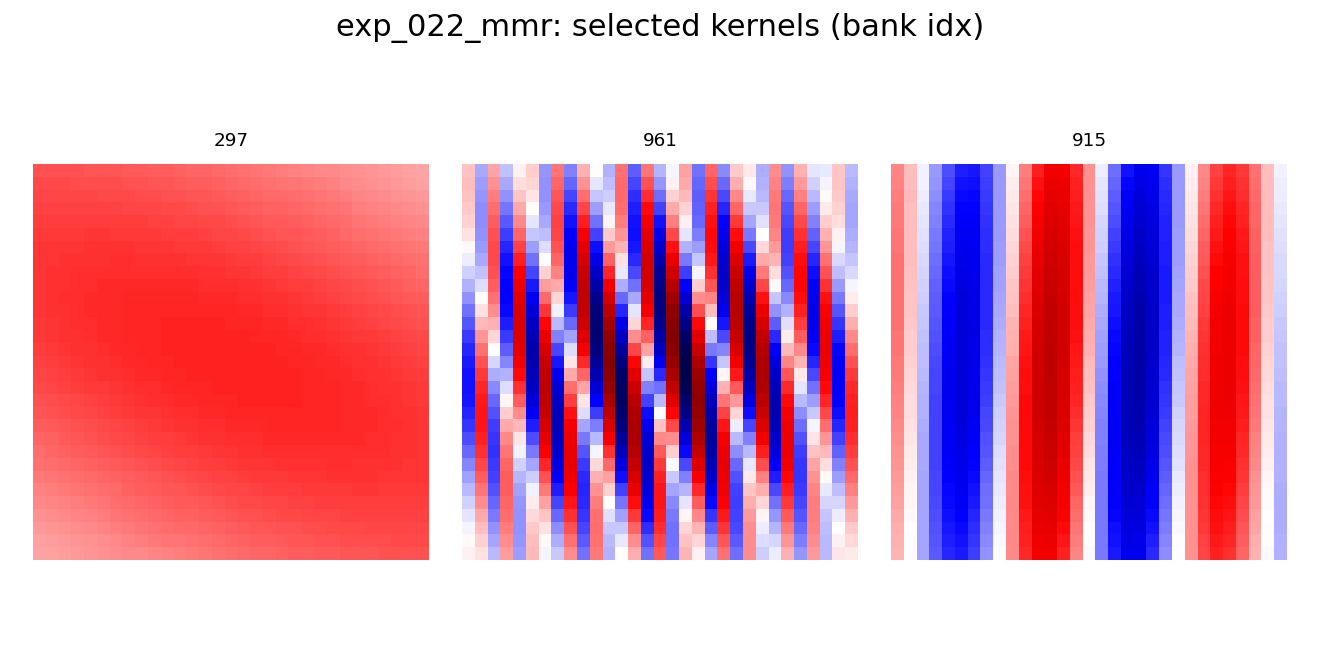
\includegraphics[width=0.98\linewidth]{figures/exp_022_mmr_selected_kernels.png}
    \caption{Selected kernels for exp\_022\_mmr (bank index shown above each kernel).}
\end{figure}

\begin{figure}[H]
    \centering
    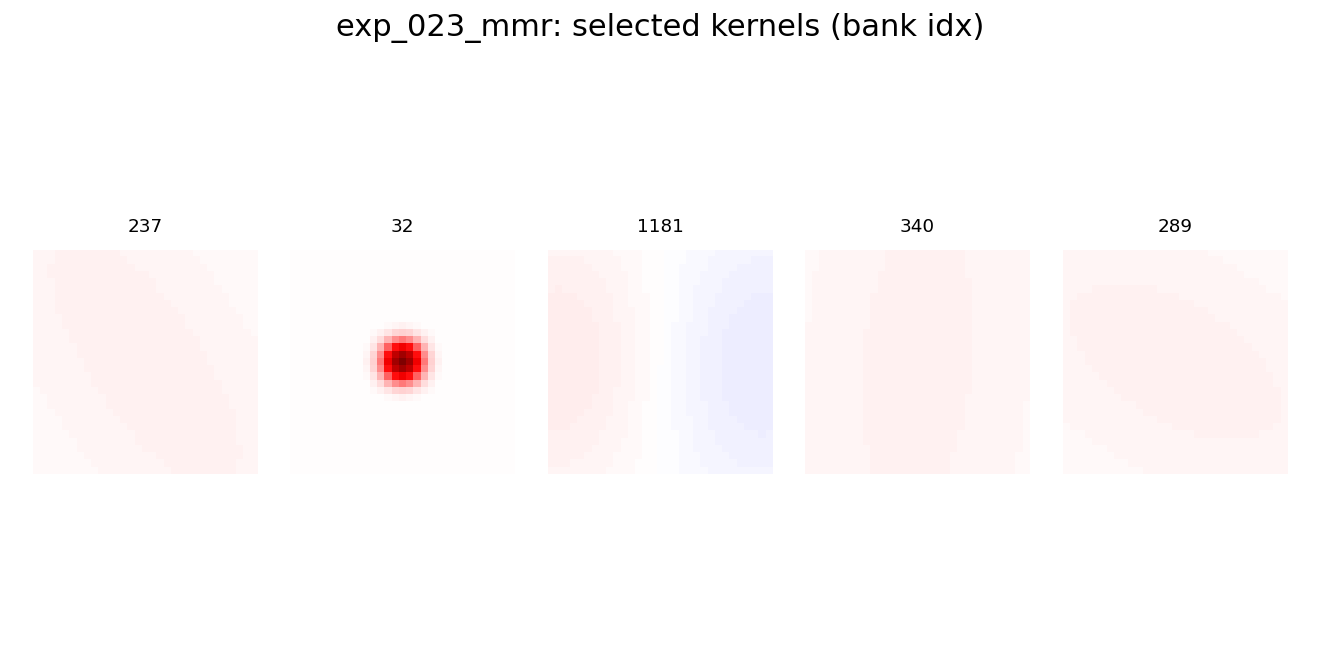
\includegraphics[width=0.98\linewidth]{figures/exp_023_mmr_selected_kernels.png}
    \caption{Selected kernels for exp\_023\_mmr (bank index shown above each kernel).}
\end{figure}

\begin{figure}[H]
    \centering
    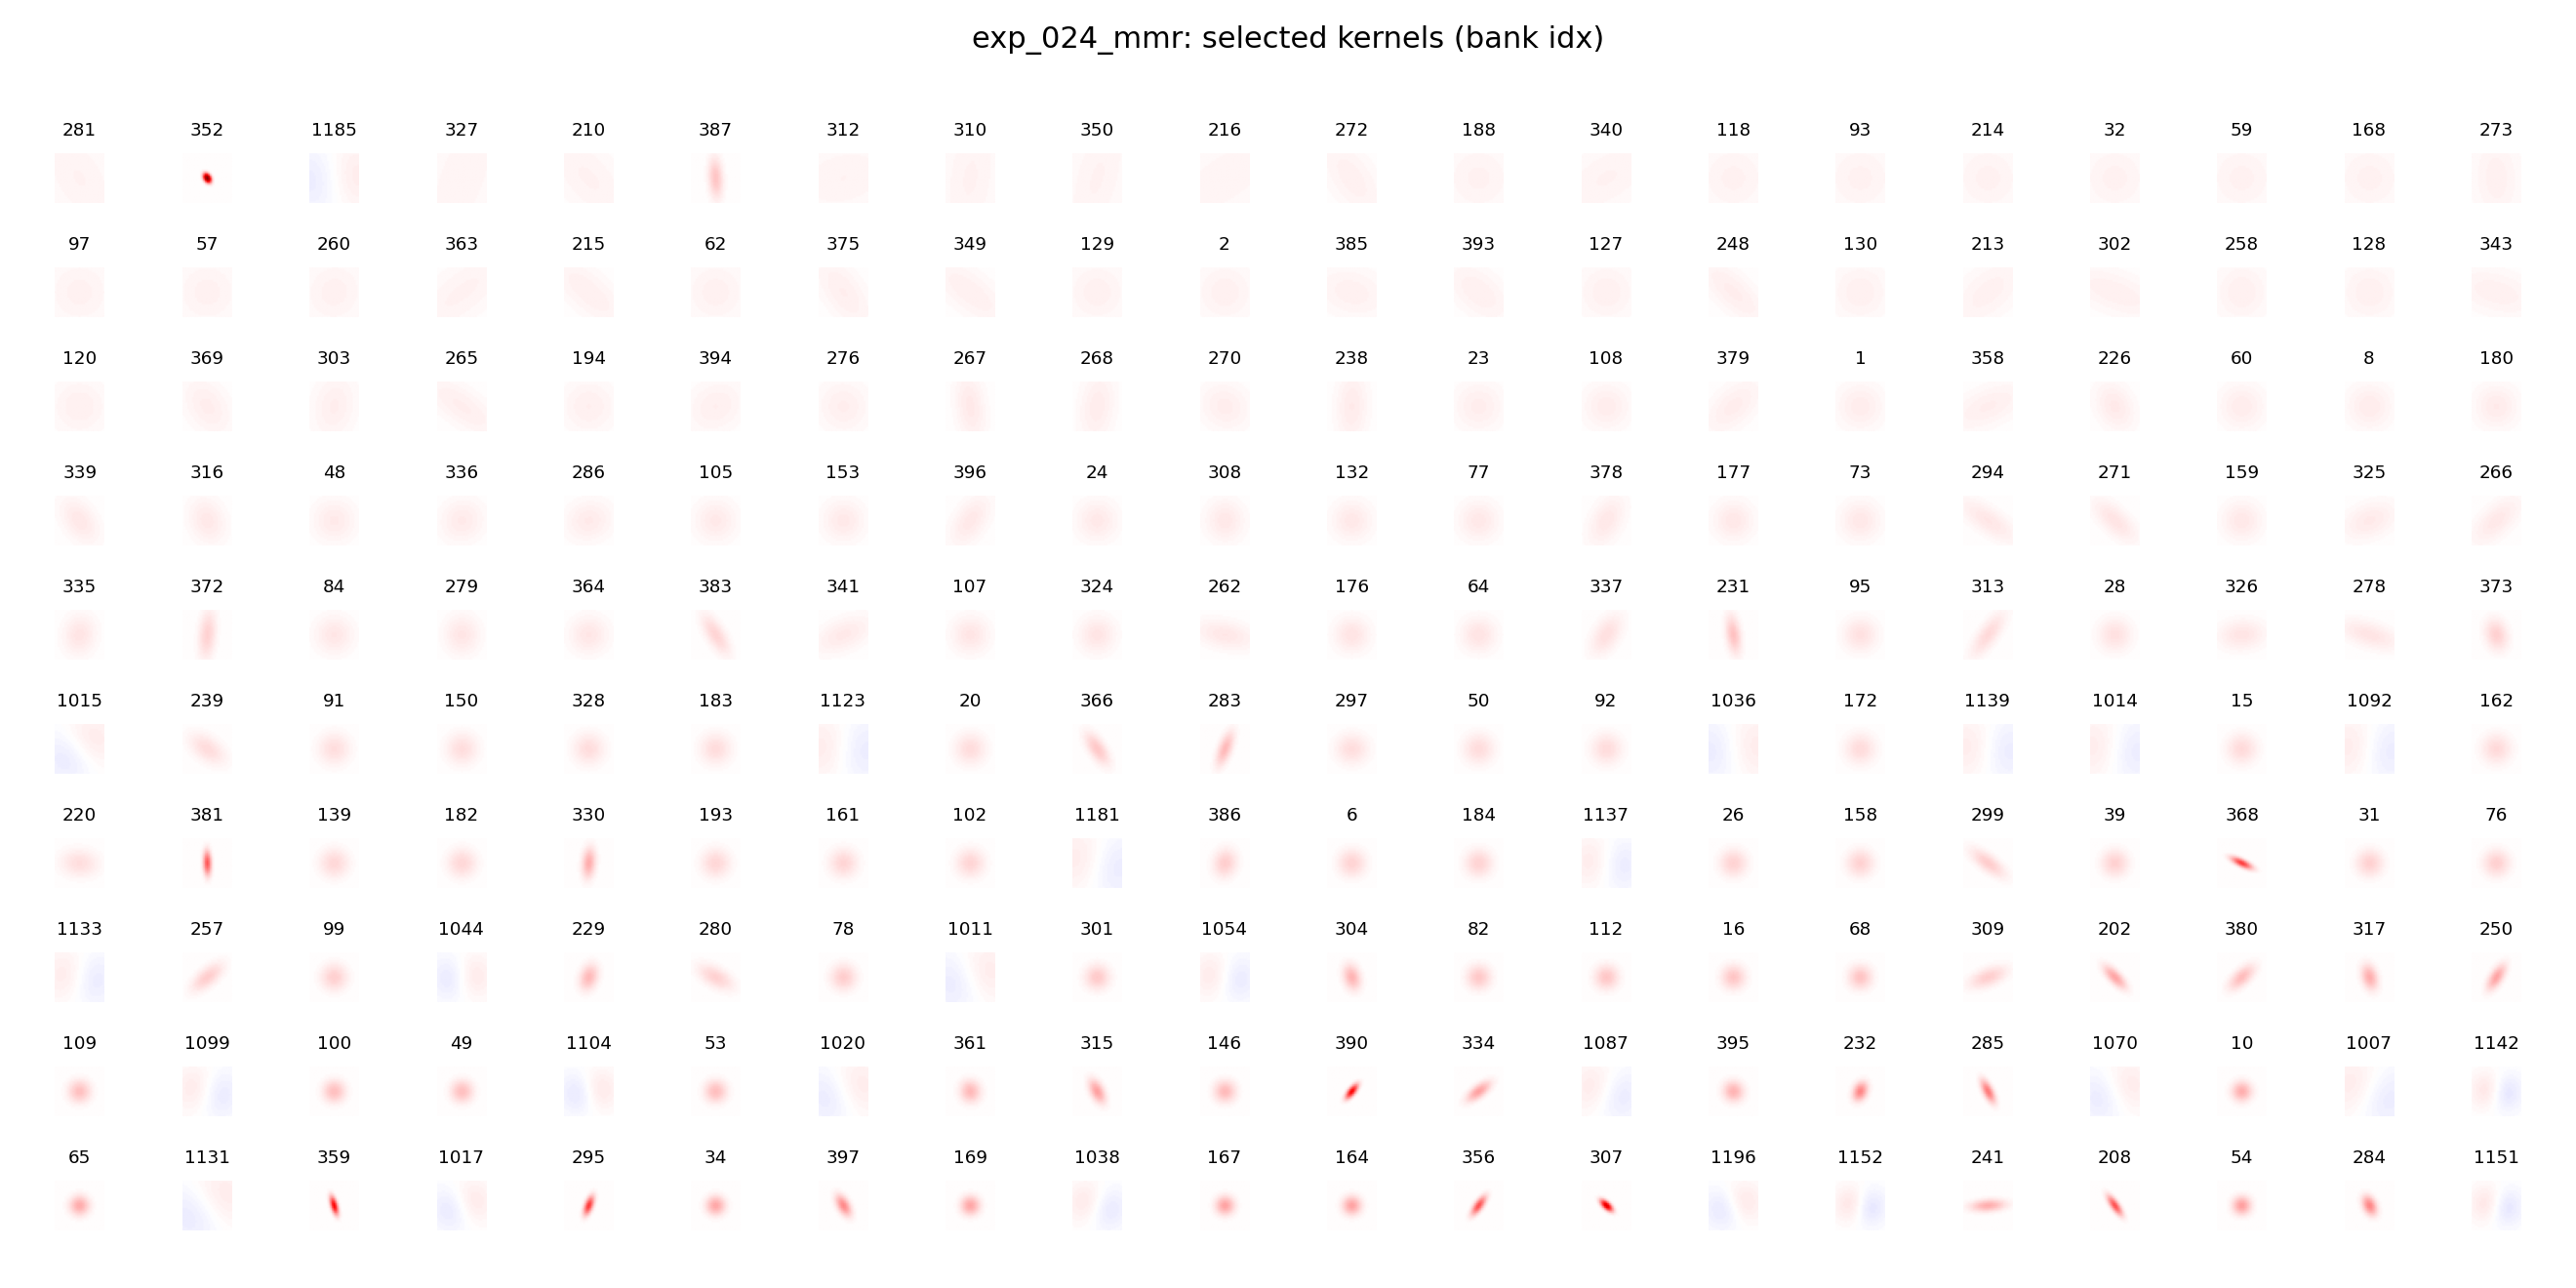
\includegraphics[width=0.98\linewidth]{figures/exp_024_mmr_selected_kernels.png}
    \caption{Selected kernels for exp\_024\_mmr (bank index shown above each kernel).}
\end{figure}

\begin{figure}[H]
    \centering
    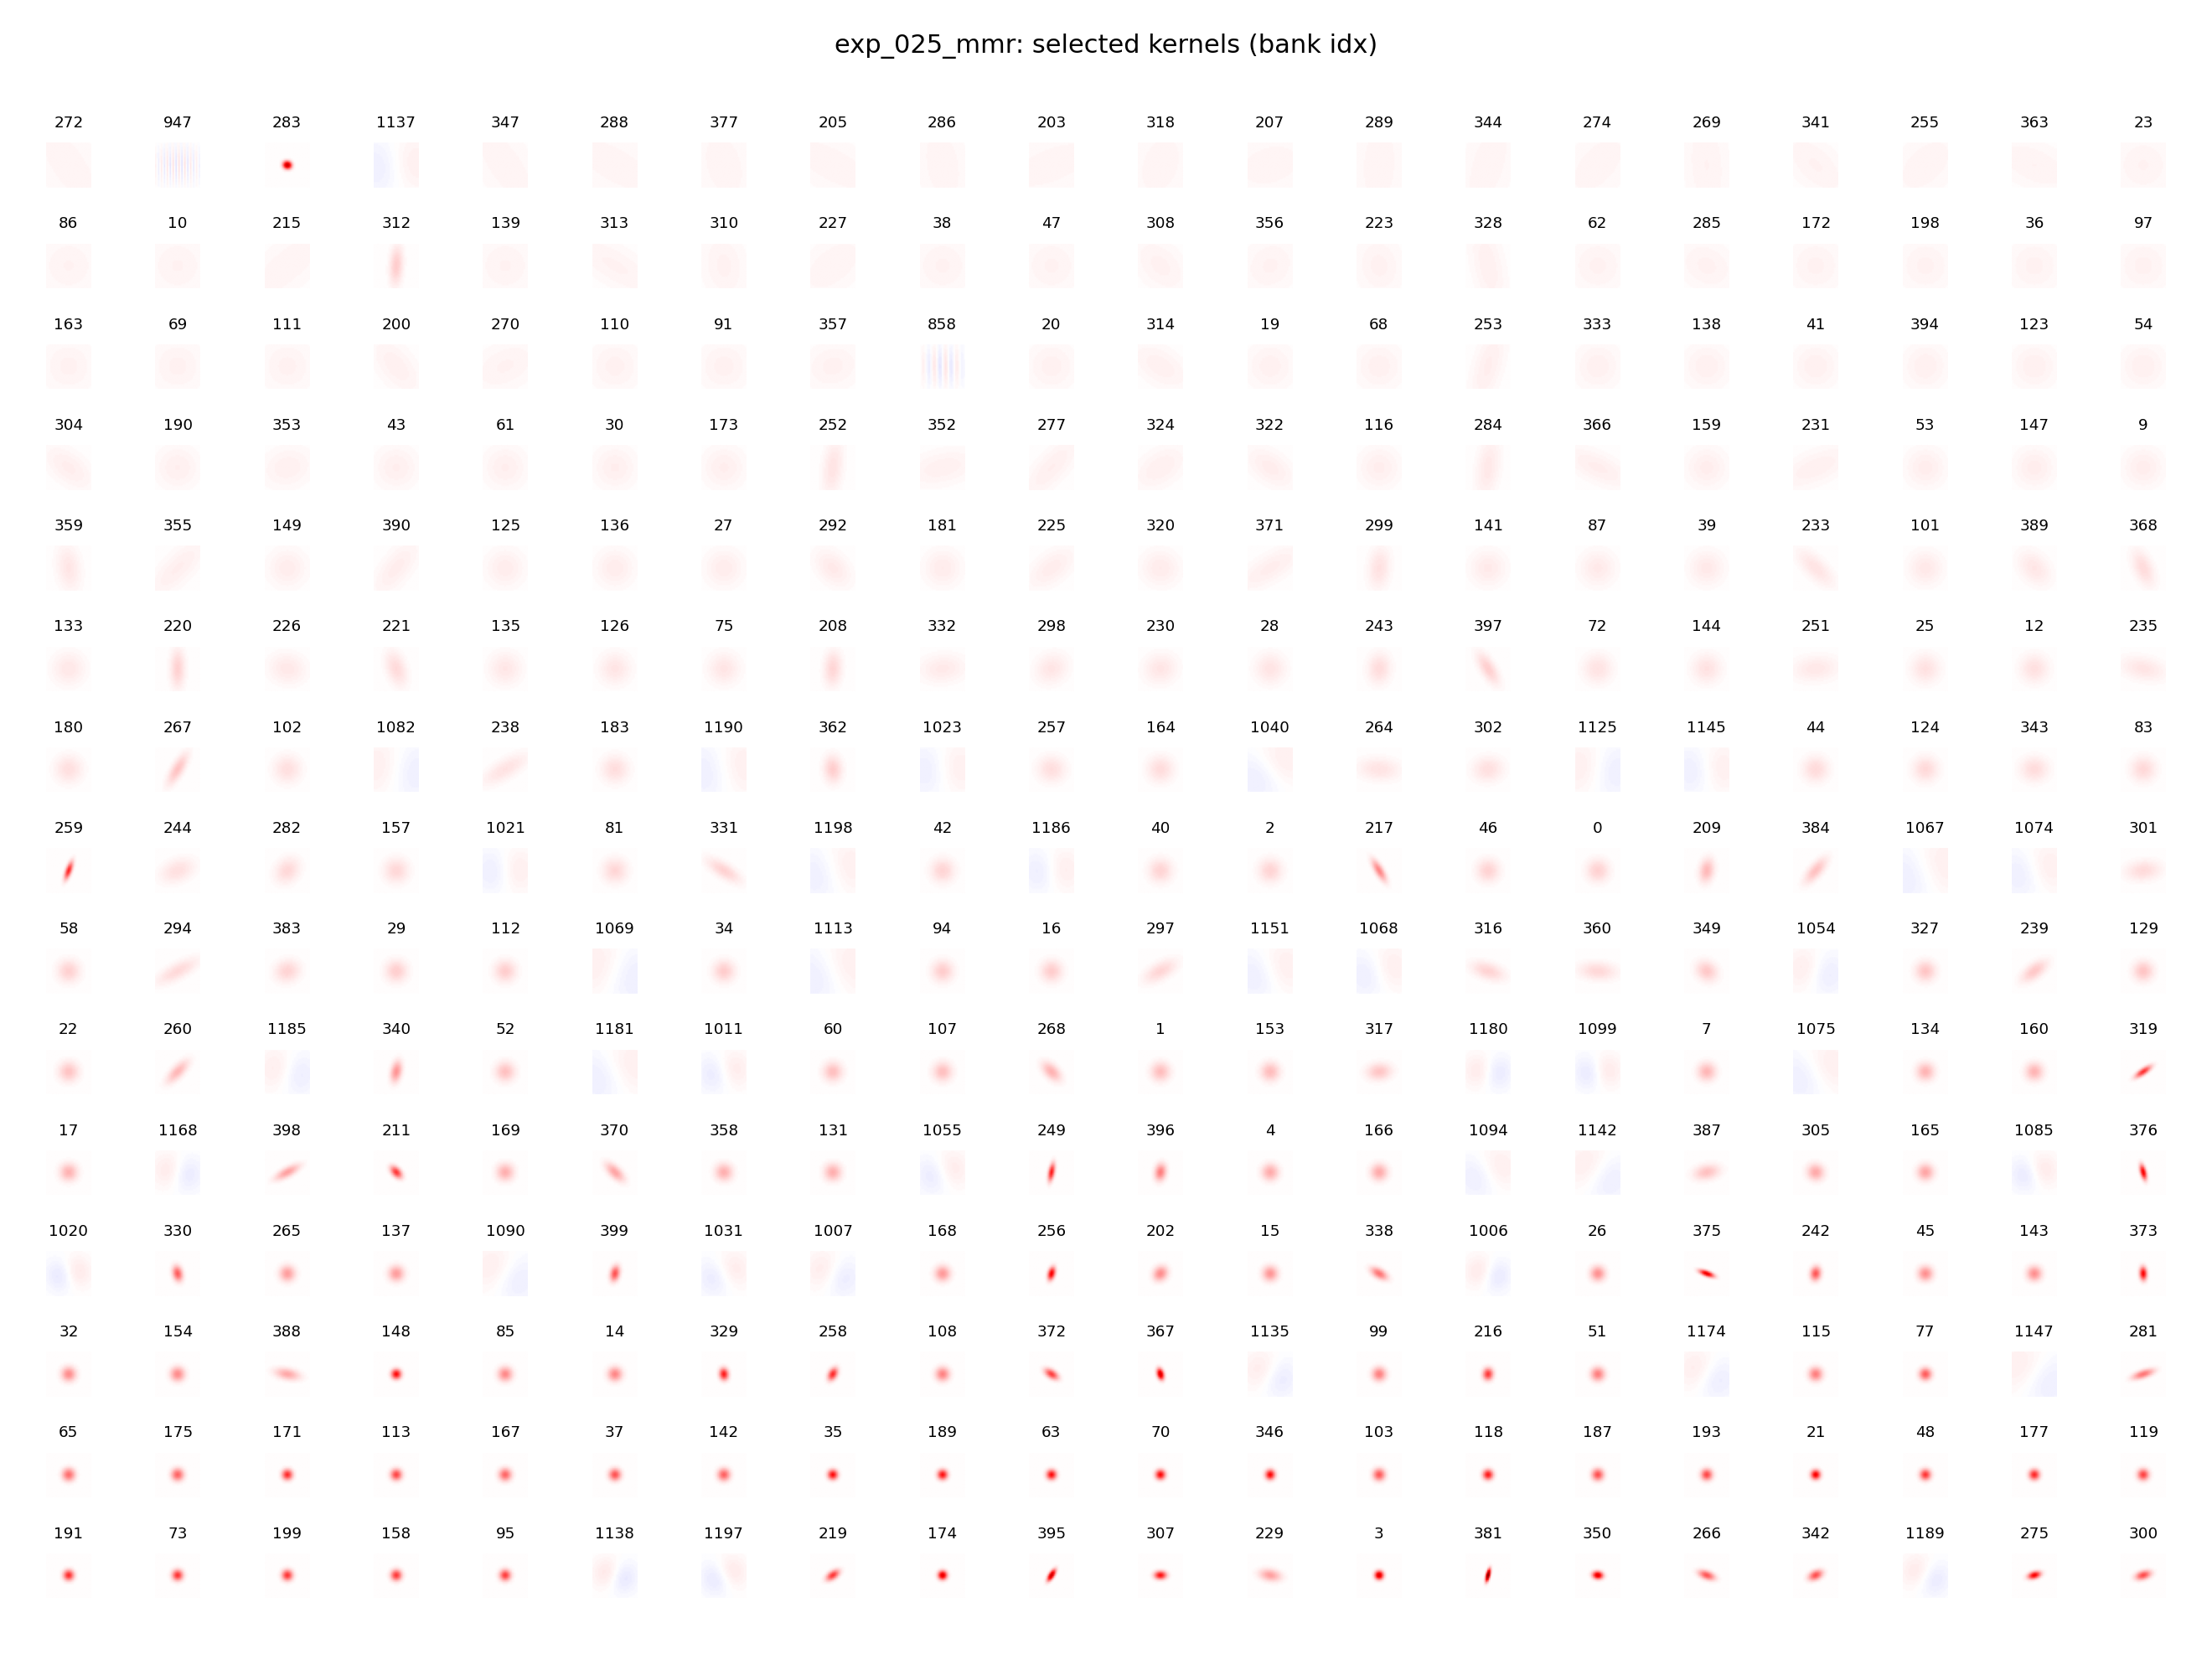
\includegraphics[width=0.98\linewidth]{figures/exp_025_mmr_selected_kernels.png}
    \caption{Selected kernels for exp\_025\_mmr (bank index shown above each kernel).}
\end{figure}

\begin{figure}[H]
    \centering
    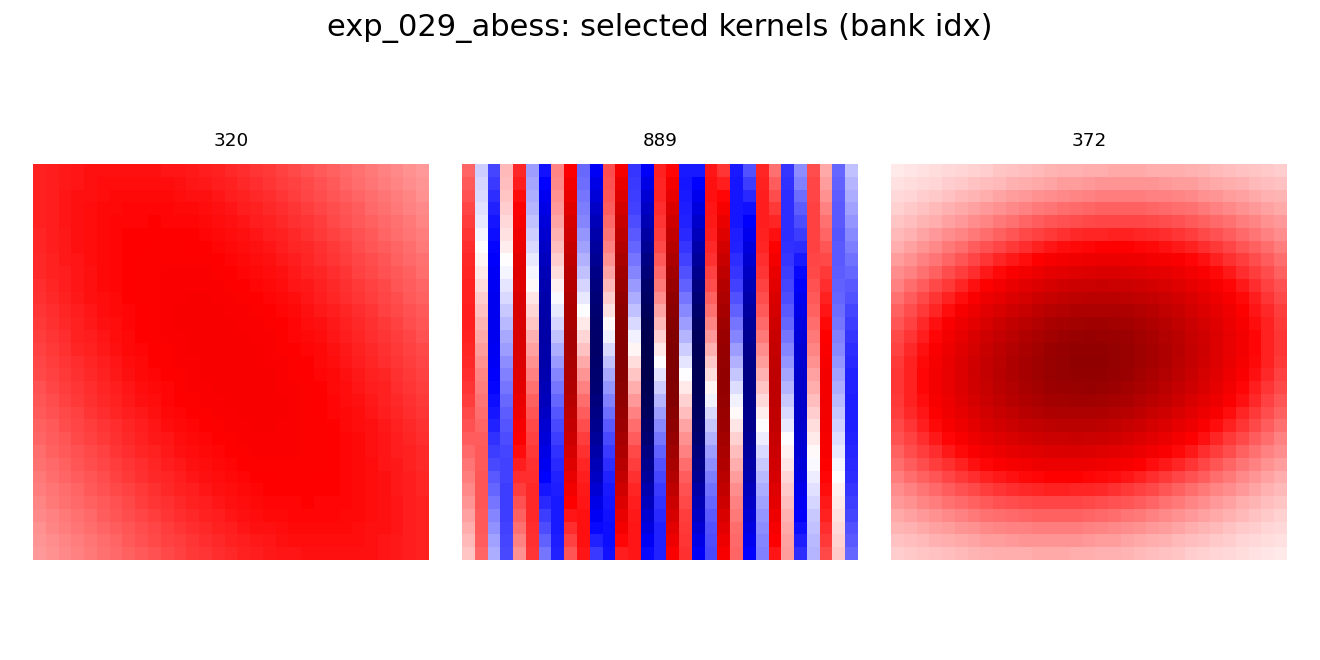
\includegraphics[width=0.98\linewidth]{figures/exp_029_abess_selected_kernels.png}
    \caption{Selected kernels for exp\_029\_abess (bank index shown above each kernel).}
\end{figure}

\begin{figure}[H]
    \centering
    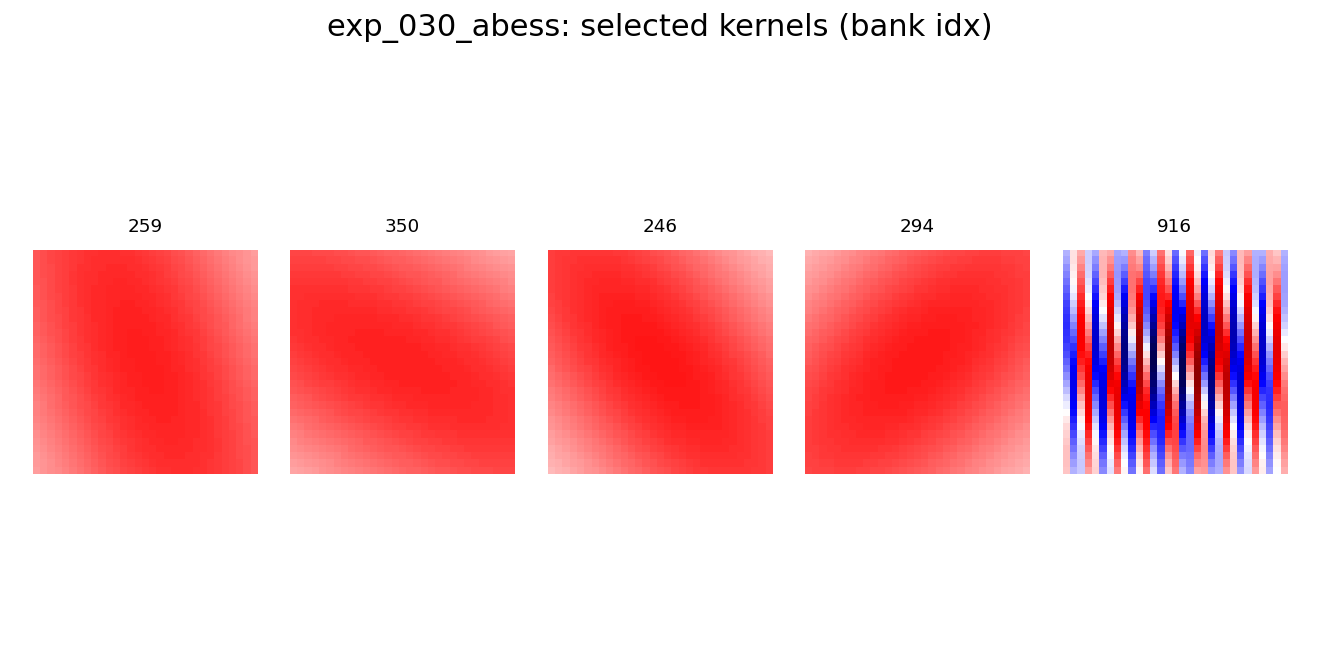
\includegraphics[width=0.98\linewidth]{figures/exp_030_abess_selected_kernels.png}
    \caption{Selected kernels for exp\_030\_abess (bank index shown above each kernel).}
\end{figure}

\begin{figure}[H]
    \centering
    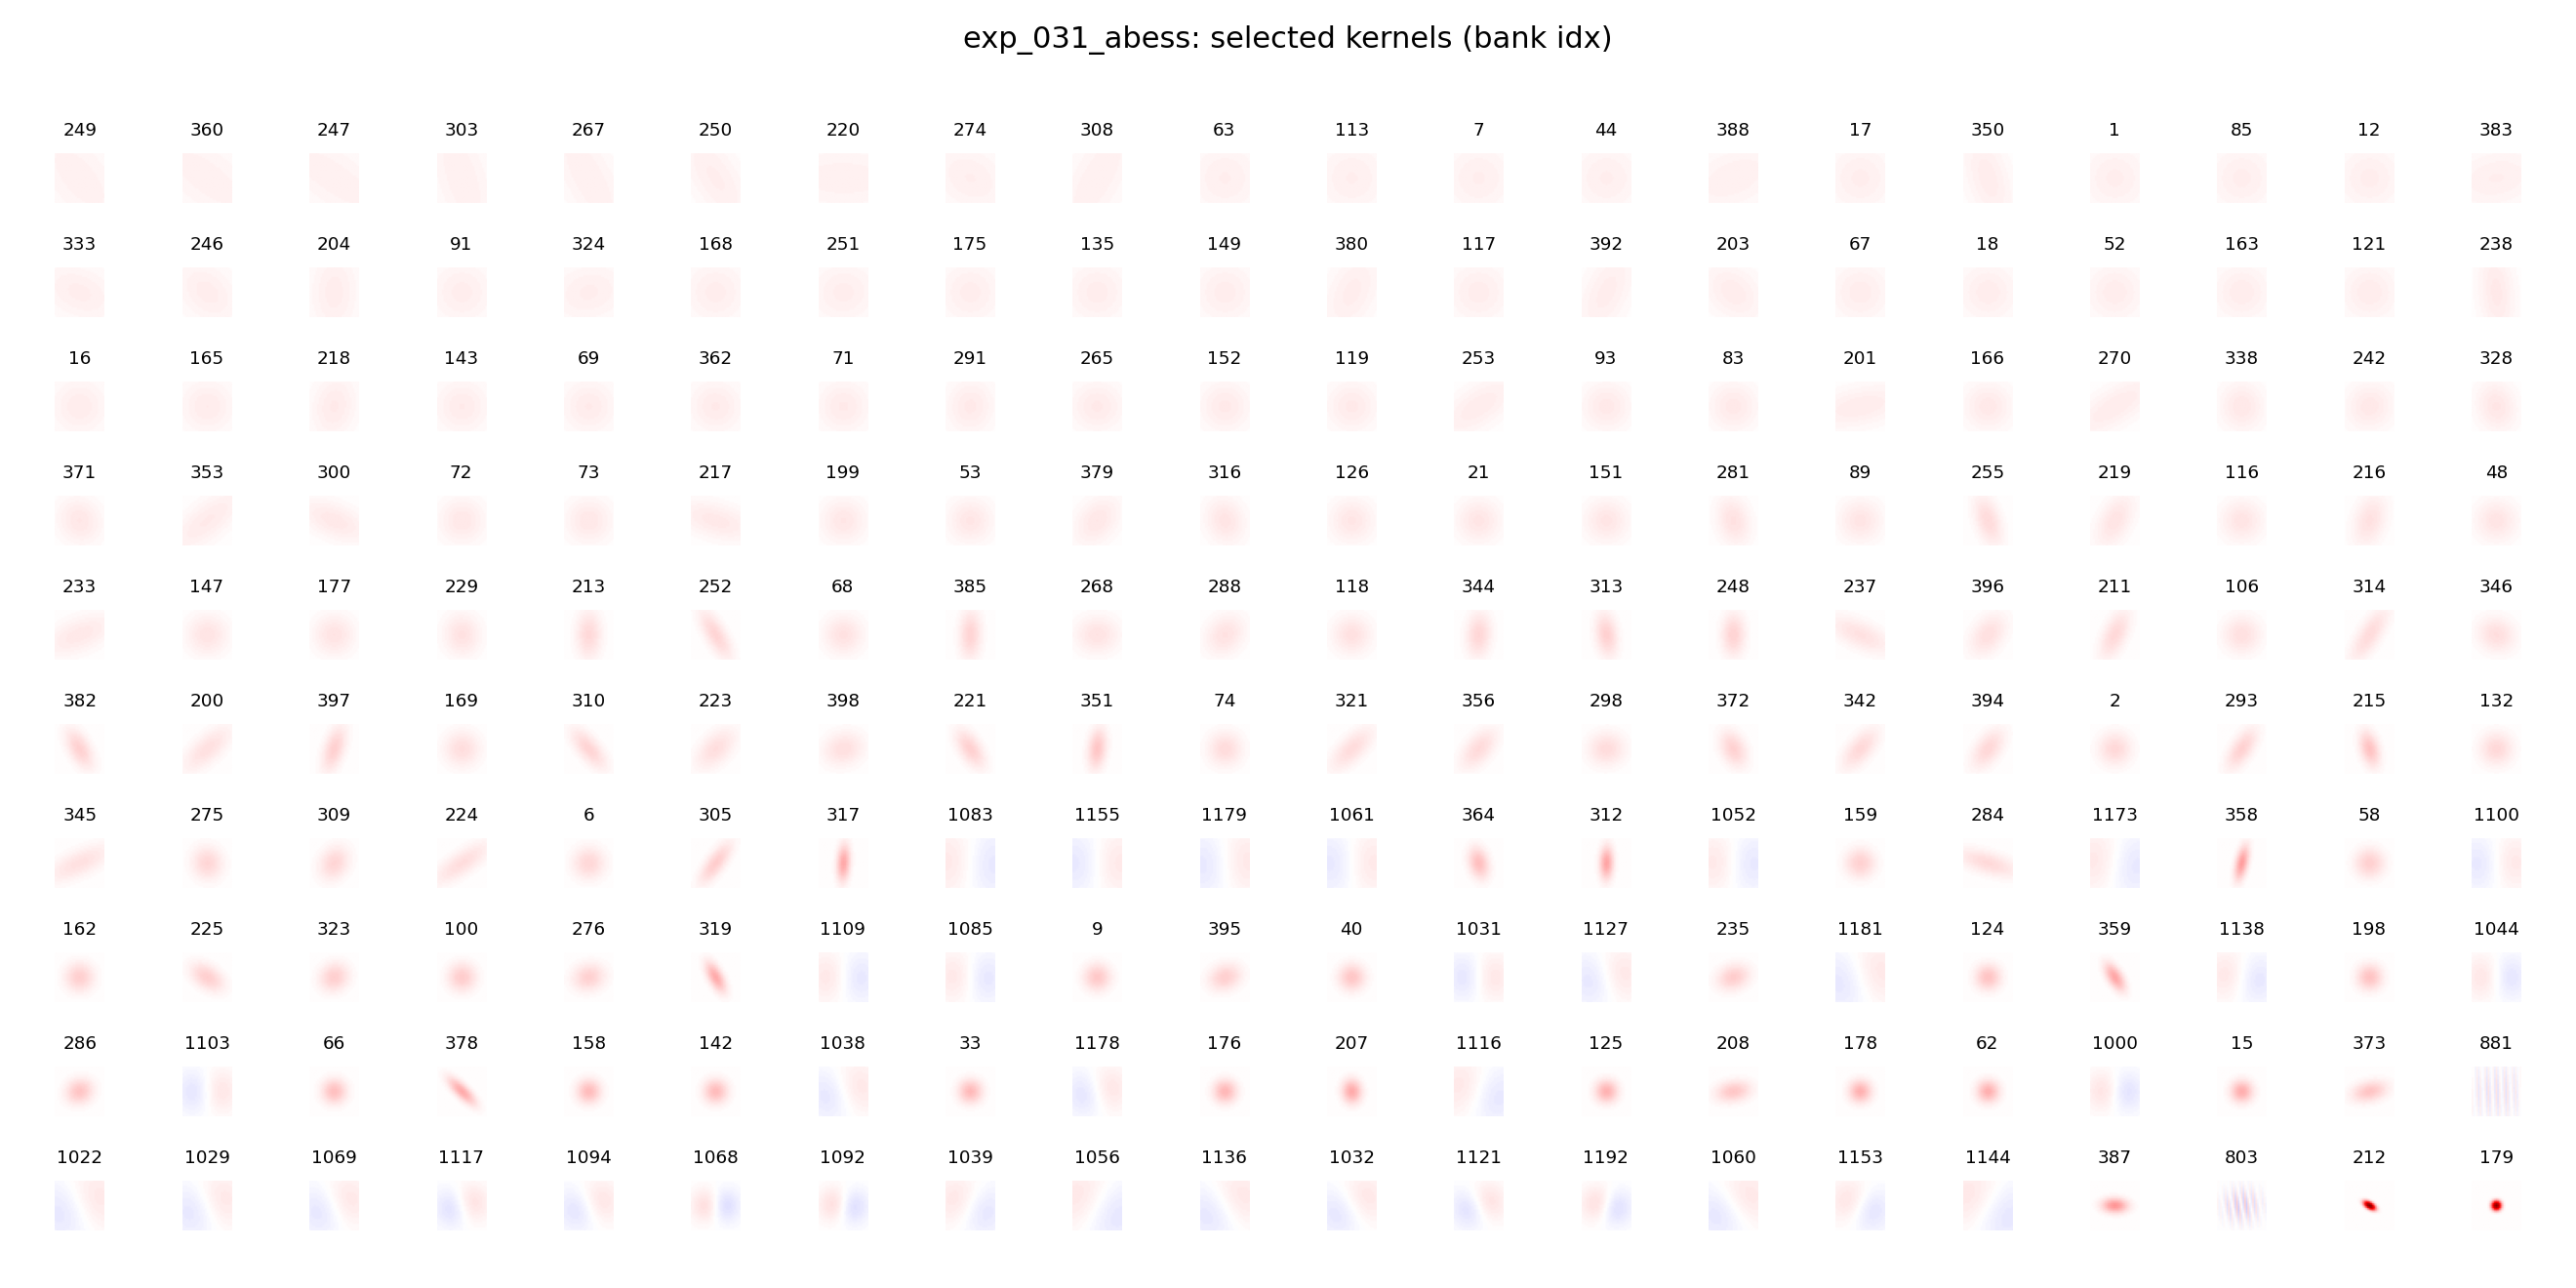
\includegraphics[width=0.98\linewidth]{figures/exp_031_abess_selected_kernels.png}
    \caption{Selected kernels for exp\_031\_abess (bank index shown above each kernel).}
\end{figure}

\begin{figure}[H]
    \centering
    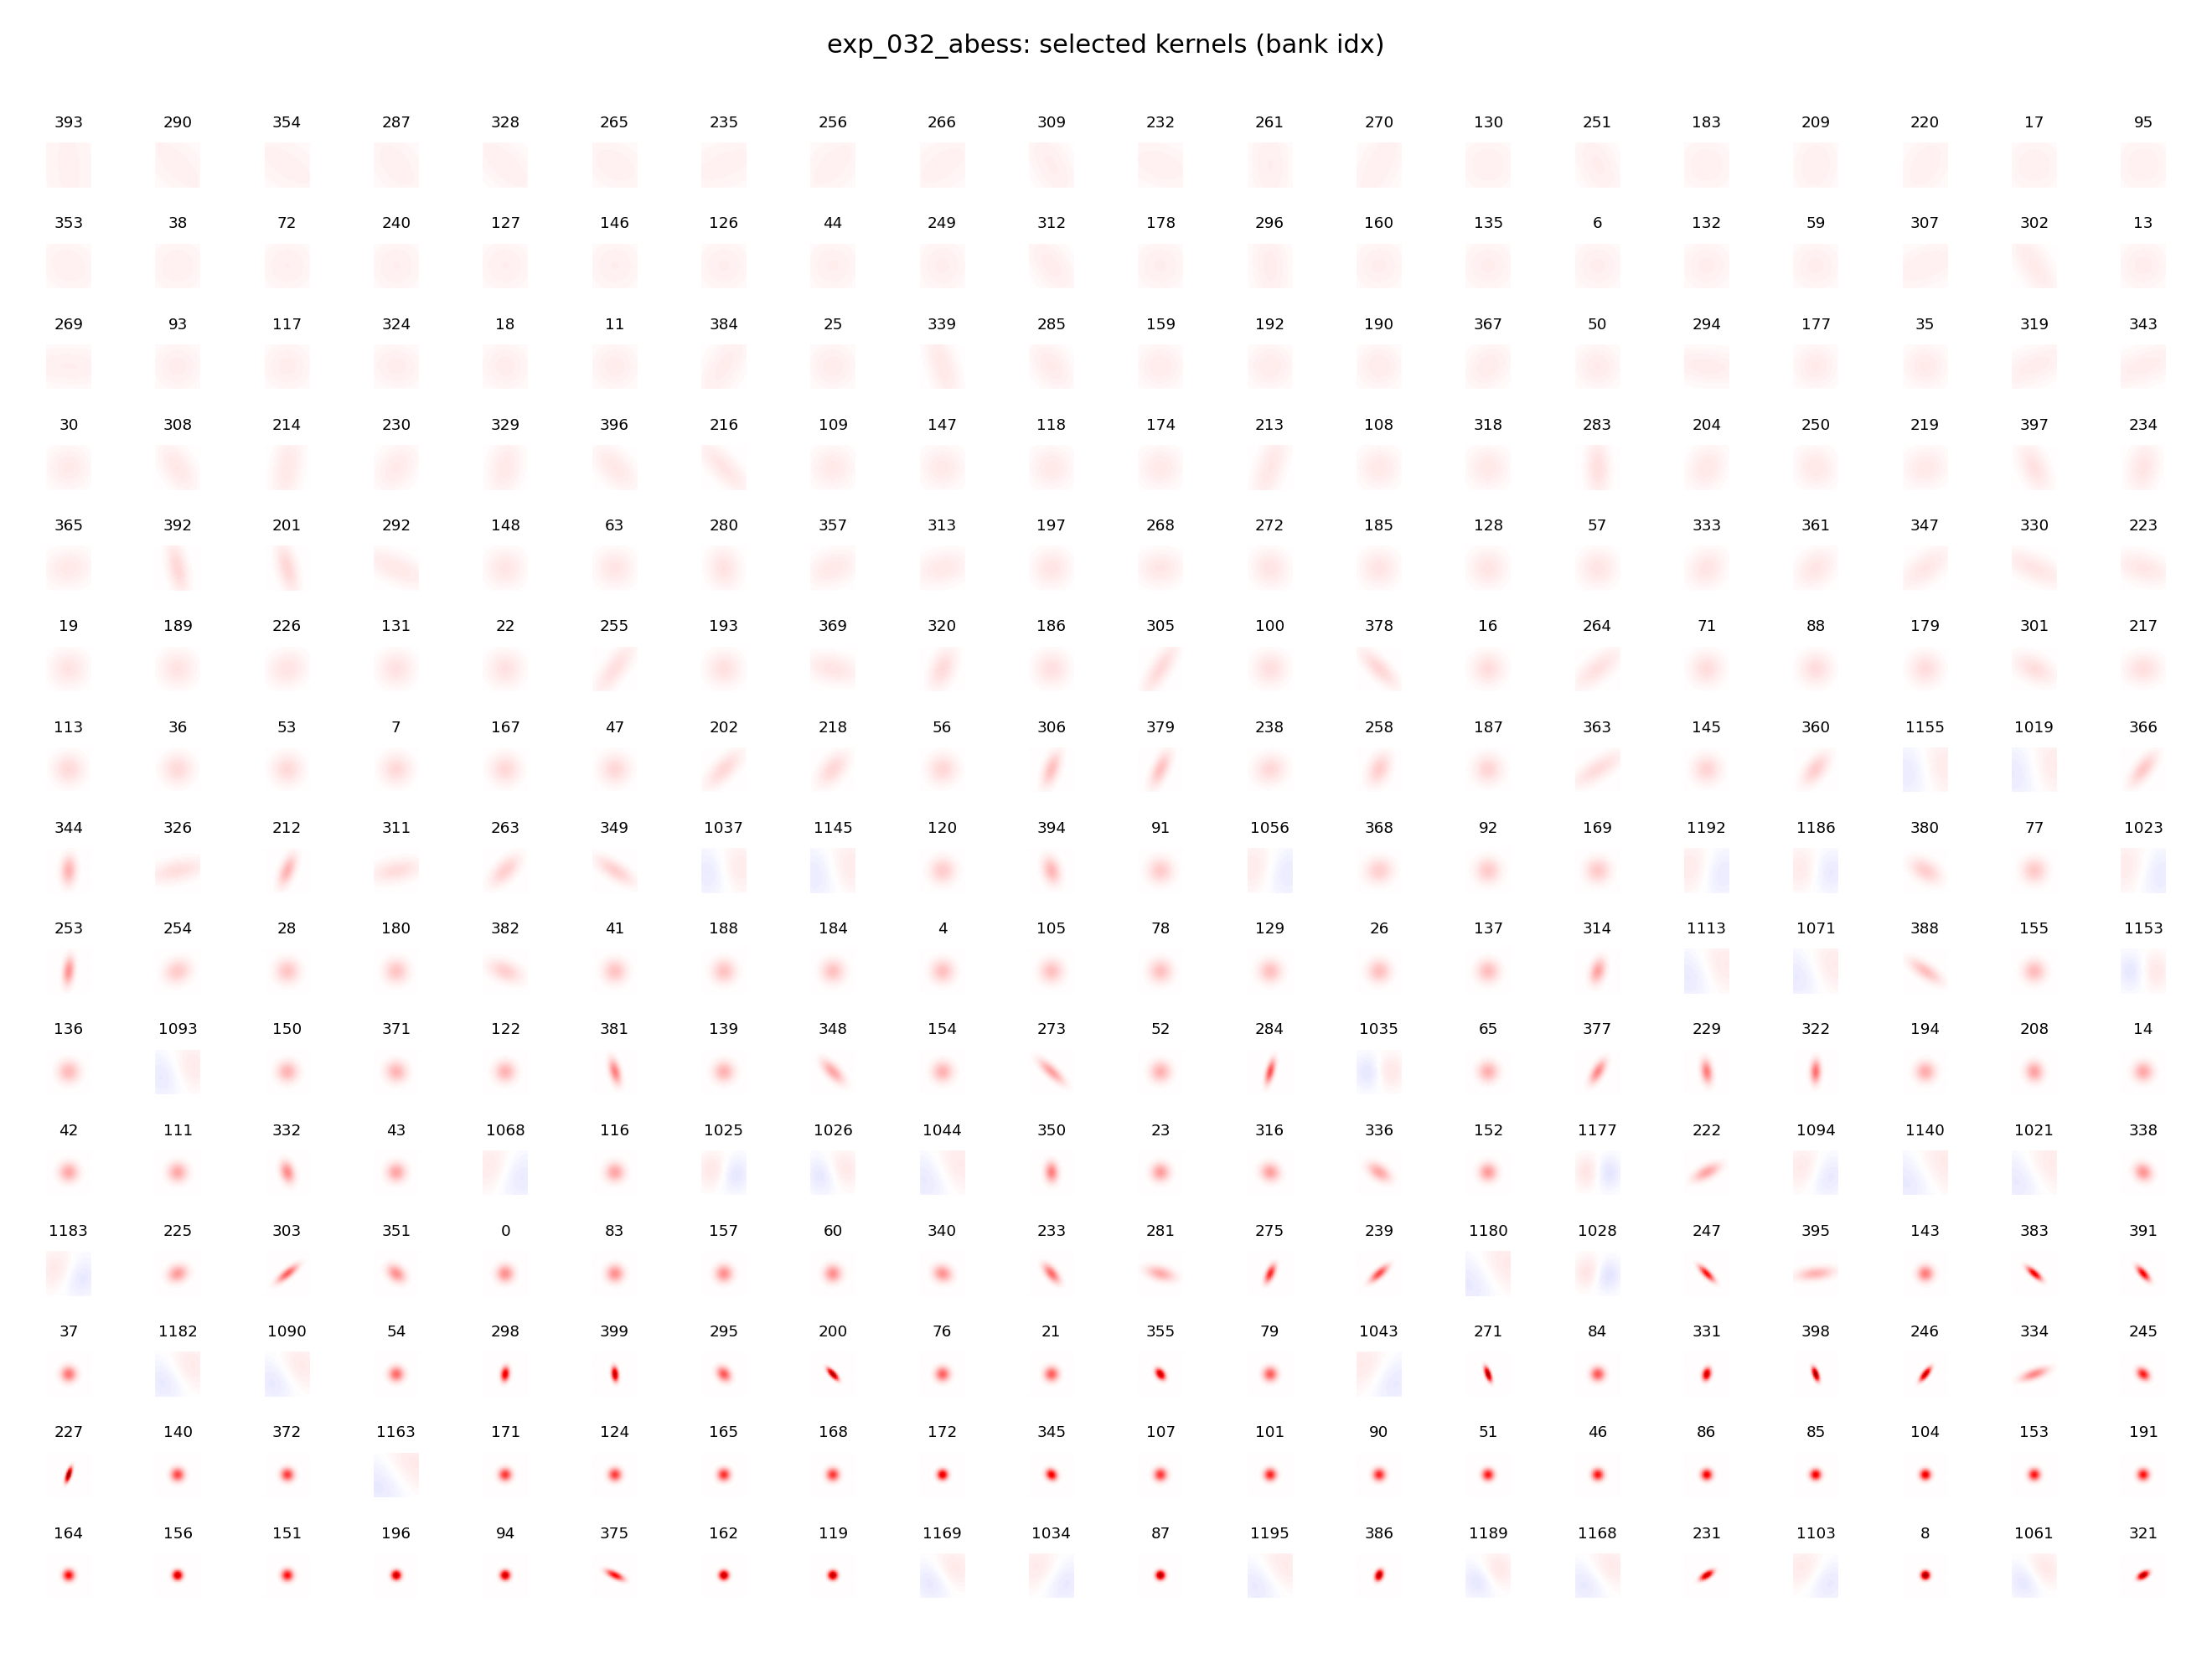
\includegraphics[width=0.98\linewidth]{figures/exp_032_abess_selected_kernels.png}
    \caption{Selected kernels for exp\_032\_abess (bank index shown above each kernel).}
\end{figure}

\clearpage
\section*{Top kernels by |weight|}
The following tables list the top 10 kernels by absolute classifier weight for each run.

\subsection*{exp\_022\_mmr}
\begin{center}
\begin{tabular}{lclllr}
\toprule
Rank & Bank idx & Family & Params (abbrev) & Sign & Weight \\
\midrule

2 & 961 & gabor & sigma=12.303, freq=0.415, theta=0.054, phase=4.144, gamma=1.249, size=31 & positive & 1.0556 \\
1 & 297 & anisotropic\_gaussian & sigma\_x=14.856, sigma\_y=38.192, theta=2.028, size=31 & positive & 0.9981 \\
3 & 915 & gabor & sigma=14.425, freq=0.072, theta=0.030, phase=1.380, gamma=0.737, size=31 & positive & 0.5509 \\
\bottomrule
\end{tabular}
\end{center}

\subsection*{exp\_023\_mmr}
\begin{center}
\begin{tabular}{lclllr}
\toprule
Rank & Bank idx & Family & Params (abbrev) & Sign & Weight \\
\midrule

4 & 340 & anisotropic\_gaussian & sigma\_x=15.104, sigma\_y=42.629, theta=0.081, size=31 & positive & 0.8677 \\
3 & 1181 & hog & sigma=14.461, theta=0.023, size=31 & positive & 0.7312 \\
5 & 289 & anisotropic\_gaussian & sigma\_x=14.655, sigma\_y=29.248, theta=2.112, size=31 & positive & 0.2675 \\
1 & 237 & anisotropic\_gaussian & sigma\_x=13.511, sigma\_y=36.080, theta=2.552, size=31 & positive & 0.0258 \\
2 & 32 & gaussian & sigma\_x=1.835, sigma\_y=1.835, theta=3.115, size=31 & positive & 0.0094 \\
\bottomrule
\end{tabular}
\end{center}

\subsection*{exp\_024\_mmr}
\begin{center}
\begin{tabular}{lclllr}
\toprule
Rank & Bank idx & Family & Params (abbrev) & Sign & Weight \\
\midrule

193 & 307 & anisotropic\_gaussian & sigma\_x=1.514, sigma\_y=3.128, theta=2.305, size=31 & negative & -0.2338 \\
2 & 352 & anisotropic\_gaussian & sigma\_x=1.421, sigma\_y=2.033, theta=2.610, size=31 & negative & -0.2202 \\
171 & 390 & anisotropic\_gaussian & sigma\_x=1.564, sigma\_y=3.657, theta=0.668, size=31 & negative & -0.2013 \\
175 & 232 & anisotropic\_gaussian & sigma\_x=4.134, sigma\_y=2.922, theta=1.976, size=31 & negative & -0.1929 \\
190 & 167 & gaussian & sigma\_x=4.029, sigma\_y=4.029, theta=2.591, size=31 & negative & -0.1695 \\
183 & 359 & anisotropic\_gaussian & sigma\_x=1.451, sigma\_y=3.932, theta=2.861, size=31 & negative & -0.1643 \\
138 & 368 & anisotropic\_gaussian & sigma\_x=1.589, sigma\_y=4.734, theta=2.017, size=31 & negative & -0.1616 \\
174 & 395 & anisotropic\_gaussian & sigma\_x=4.484, sigma\_y=4.367, theta=0.759, size=31 & negative & -0.1589 \\
157 & 202 & anisotropic\_gaussian & sigma\_x=2.558, sigma\_y=6.329, theta=2.368, size=31 & negative & -0.1555 \\
199 & 284 & anisotropic\_gaussian & sigma\_x=2.767, sigma\_y=4.380, theta=2.711, size=31 & negative & -0.1544 \\
\bottomrule
\end{tabular}
\end{center}

\subsection*{exp\_025\_mmr}
\begin{center}
\begin{tabular}{lclllr}
\toprule
Rank & Bank idx & Family & Params (abbrev) & Sign & Weight \\
\midrule

289 & 174 & gaussian & sigma\_x=2.071, sigma\_y=2.071, theta=1.774, size=31 & negative & -0.2016 \\
3 & 283 & anisotropic\_gaussian & sigma\_x=1.793, sigma\_y=2.001, theta=1.804, size=31 & negative & -0.2012 \\
290 & 395 & anisotropic\_gaussian & sigma\_x=1.262, sigma\_y=2.909, theta=0.560, size=31 & negative & -0.1980 \\
251 & 367 & anisotropic\_gaussian & sigma\_x=1.533, sigma\_y=2.587, theta=2.873, size=31 & negative & -0.1935 \\
299 & 275 & anisotropic\_gaussian & sigma\_x=1.646, sigma\_y=2.978, theta=1.300, size=31 & negative & -0.1825 \\
49 & 858 & gabor & sigma=11.845, freq=0.130, theta=3.133, phase=1.695, gamma=1.221, size=31 & positive & 0.1771 \\
270 & 63 & gaussian & sigma\_x=2.302, sigma\_y=2.302, theta=0.141, size=31 & negative & -0.1743 \\
280 & 119 & gaussian & sigma\_x=2.626, sigma\_y=2.626, theta=1.881, size=31 & negative & -0.1702 \\
11 & 318 & anisotropic\_gaussian & sigma\_x=14.402, sigma\_y=23.362, theta=0.320, size=31 & positive & 0.1690 \\
10 & 203 & anisotropic\_gaussian & sigma\_x=14.816, sigma\_y=39.076, theta=1.204, size=31 & positive & 0.1683 \\
\bottomrule
\end{tabular}
\end{center}

\subsection*{exp\_029\_abess}
\begin{center}
\begin{tabular}{lclllr}
\toprule
Rank & Bank idx & Family & Params (abbrev) & Sign & Weight \\
\midrule

3 & 372 & anisotropic\_gaussian & sigma\_x=11.561, sigma\_y=7.902, theta=2.940, size=31 & positive & 0.7198 \\
1 & 320 & anisotropic\_gaussian & sigma\_x=14.951, sigma\_y=37.142, theta=2.537, size=31 & positive & 0.3697 \\
2 & 889 & gabor & sigma=12.113, freq=0.255, theta=3.112, phase=1.578, gamma=0.736, size=31 & positive & 0.3197 \\
\bottomrule
\end{tabular}
\end{center}

\subsection*{exp\_030\_abess}
\begin{center}
\begin{tabular}{lclllr}
\toprule
Rank & Bank idx & Family & Params (abbrev) & Sign & Weight \\
\midrule

2 & 350 & anisotropic\_gaussian & sigma\_x=15.312, sigma\_y=44.003, theta=2.073, size=31 & positive & 0.6834 \\
5 & 916 & gabor & sigma=14.013, freq=0.263, theta=3.090, phase=4.547, gamma=1.460, size=31 & positive & 0.4490 \\
1 & 259 & anisotropic\_gaussian & sigma\_x=15.129, sigma\_y=40.973, theta=2.769, size=31 & positive & 0.4041 \\
3 & 246 & anisotropic\_gaussian & sigma\_x=13.684, sigma\_y=34.884, theta=2.458, size=31 & positive & 0.3703 \\
4 & 294 & anisotropic\_gaussian & sigma\_x=14.403, sigma\_y=31.963, theta=0.795, size=31 & positive & 0.2061 \\
\bottomrule
\end{tabular}
\end{center}

\subsection*{exp\_031\_abess}
\begin{center}
\begin{tabular}{lclllr}
\toprule
Rank & Bank idx & Family & Params (abbrev) & Sign & Weight \\
\midrule

199 & 212 & anisotropic\_gaussian & sigma\_x=2.611, sigma\_y=1.372, theta=0.543, size=31 & negative & -0.2458 \\
200 & 179 & gaussian & sigma\_x=1.929, sigma\_y=1.929, theta=0.542, size=31 & negative & -0.2216 \\
197 & 387 & anisotropic\_gaussian & sigma\_x=3.175, sigma\_y=5.504, theta=1.605, size=31 & negative & -0.1909 \\
157 & 359 & anisotropic\_gaussian & sigma\_x=3.129, sigma\_y=6.639, theta=2.594, size=31 & negative & -0.1453 \\
175 & 178 & gaussian & sigma\_x=4.833, sigma\_y=4.833, theta=0.030, size=31 & negative & -0.1447 \\
3 & 247 & anisotropic\_gaussian & sigma\_x=13.770, sigma\_y=40.930, theta=2.170, size=31 & positive & 0.1352 \\
24 & 91 & gaussian & sigma\_x=13.807, sigma\_y=13.807, theta=1.855, size=31 & positive & 0.1350 \\
7 & 220 & anisotropic\_gaussian & sigma\_x=14.050, sigma\_y=33.972, theta=1.584, size=31 & positive & 0.1334 \\
13 & 44 & gaussian & sigma\_x=15.181, sigma\_y=15.181, theta=0.638, size=31 & positive & 0.1333 \\
32 & 117 & gaussian & sigma\_x=13.372, sigma\_y=13.372, theta=3.007, size=31 & positive & 0.1326 \\
\bottomrule
\end{tabular}
\end{center}

\subsection*{exp\_032\_abess}
\begin{center}
\begin{tabular}{lclllr}
\toprule
Rank & Bank idx & Family & Params (abbrev) & Sign & Weight \\
\midrule

288 & 119 & gaussian & sigma\_x=2.039, sigma\_y=2.039, theta=2.935, size=31 & negative & -0.2167 \\
287 & 162 & gaussian & sigma\_x=2.098, sigma\_y=2.098, theta=1.138, size=31 & negative & -0.1893 \\
257 & 398 & anisotropic\_gaussian & sigma\_x=1.240, sigma\_y=2.948, theta=2.801, size=31 & negative & -0.1889 \\
284 & 196 & gaussian & sigma\_x=2.142, sigma\_y=2.142, theta=0.274, size=31 & negative & -0.1872 \\
251 & 355 & anisotropic\_gaussian & sigma\_x=2.658, sigma\_y=1.767, theta=0.950, size=31 & negative & -0.1871 \\
274 & 51 & gaussian & sigma\_x=2.674, sigma\_y=2.674, theta=0.687, size=31 & negative & -0.1797 \\
279 & 153 & gaussian & sigma\_x=2.634, sigma\_y=2.634, theta=2.281, size=31 & negative & -0.1794 \\
300 & 321 & anisotropic\_gaussian & sigma\_x=2.653, sigma\_y=1.500, theta=2.616, size=31 & negative & -0.1768 \\
246 & 399 & anisotropic\_gaussian & sigma\_x=1.445, sigma\_y=3.069, theta=3.035, size=31 & negative & -0.1745 \\
285 & 94 & gaussian & sigma\_x=2.172, sigma\_y=2.172, theta=2.690, size=31 & negative & -0.1724 \\
\bottomrule
\end{tabular}
\end{center}

\end{document}
